
\documentclass[9pt]{beamer}

\usepackage[latin1]{inputenc}
\usepackage{colortbl}
\usepackage[english]{babel}

\newcommand{\myblue} [1] {{\color{blue}#1}}
\newcommand{\newauthor}[4]{
  \parbox{0.26\textwidth}{
    \texorpdfstring
      {
        \centering
        #1 \\
        \myblue{{\href{#2}{\texttt{#3}}}} \\
        #4 \\
      }
      {#1}
  }
}



% beamer template
\beamertemplatetransparentcovereddynamic
\usetheme{default}

\hypersetup{%
  pdftitle={Go-HEP},%
   pdfauthor={Sebastien Binet},%
%
}

\title[Go-HEP]{Go-HEP}
\author[Sebastien Binet]{
 \parbox{0.26\textwidth}{
	\texorpdfstring
	  {
		\centering
 		Sebastien Binet \\
 		CNRS/IN2P3/LPC-Clermont \\
 		\myblue{\href{https://github.com/sbinet}{\texttt{https://github.com/sbinet}}} \\
 		\myblue{\href{http://twitter.com/0xbins}{\texttt{@0xbins}}} \\
 		\myblue{\href{mailto:binet@cern.ch}{\texttt{binet@cern.ch}}} \\
 	  }
	{Sebastien Binet}
}
 }



\begin{document}

\frame{\titlepage
}

\part<presentation>{Main Talk}

\section[slides]{slides}

\begin{frame}[fragile]
\frametitle{Go-HEP}


	\emph{"Software is complicated."}

Compilation/D\'eveloppement/D\'eploiement de code C++/Python: compliqu\'e

\begin{itemize}
\item \texttt{C++/ROOT}: rapide \`a l'ex\'ecution, lent \`a d\'evelopper (programmation multi-thread\'ee pas ais\'ee)
\item \texttt{Python}: d\'eveloppement rapide \& intuitif, lent \`a l'ex\'ecution, peu maintenable
\end{itemize}

\myblue{\href{https://go-hep.org}{\texttt{Go-HEP}}}: une biblioth\`eque \'ecrite en \myblue{\href{https://golang.org}{\texttt{Go}}} pour \'ecrire des analyses de donn\'ees.


\begin{itemize}
\item \texttt{Go} est compil\'e, facilement d\'eployable, compilable rapidement
\item d\'ependances install\'ees automatiquement (Linux/macOS/Windows)
\item support pour la programmation parall\`ele
\end{itemize}

\texttt{Go-HEP}:


\begin{itemize}
\item lecture de fichiers ROOT (\'ecriture: \textbf{bient\^ot})
\item histogrammes, scatter, plots, n-tuples, fits, 4-vector
\item LCIO, LHEF, HepMC, HEPEVT, HepPDT, CSV, SLHA, 
\item xrootd
\item \myblue{\texttt{Gonum}}: Calcul matriciel, distributions, FFT, \ldots
\end{itemize}


\end{frame}

\begin{frame}[fragile]
\frametitle{Go-HEP}

\begin{figure}[h]
\begin{center}
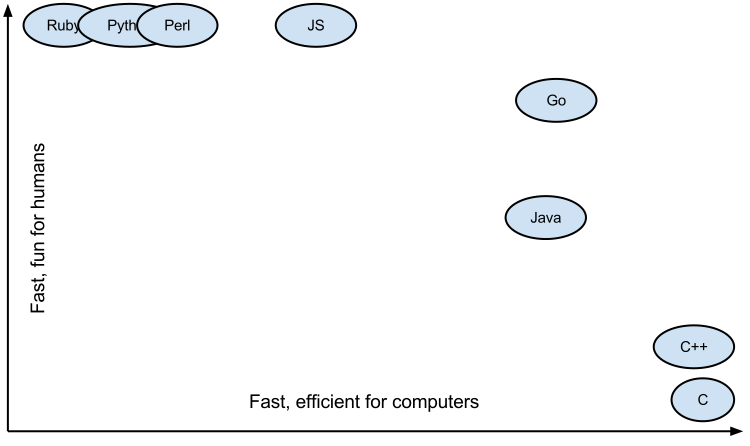
\includegraphics[width=\textwidth]{_figs/funfast.png}
\end{center}

\end{figure}

\end{frame}


\end{document}
